\documentclass{article}



% This document contains the TikZ-header for all our LaTeX-computations.
% It especially contains all global graphic parameters.

\usepackage{amsmath, amssymb, amsfonts} % Standard Math-stuff

\usepackage{tikz}
\usetikzlibrary{calc}
\usetikzlibrary{positioning}
\usetikzlibrary{shapes}
\usetikzlibrary{patterns}

% Define a text=none option for nodes that ignores the given text, from
% https://tex.stackexchange.com/questions/59354/no-text-none-in-tikz
\makeatletter
\newif\iftikz@node@phantom
\tikzset{
  phantom/.is if=tikz@node@phantom,
  text/.code=%
    \edef\tikz@temp{#1}%
    \ifx\tikz@temp\tikz@nonetext
      \tikz@node@phantomtrue
    \else
      \tikz@node@phantomfalse
      \let\tikz@textcolor\tikz@temp
    \fi
}
\usepackage{etoolbox}
\patchcmd\tikz@fig@continue{\tikz@node@transformations}{%
  \iftikz@node@phantom
    \setbox\pgfnodeparttextbox\hbox{}
  \fi\tikz@node@transformations}{}{}
\makeatother

% Now we define the global styles
% The global styles are defined nestedly. You have to give your tikzpicture
% the global options [vertexStyle, edgeStyle, faceStyle] to activate them.
% 
% You can disable labels by using the option nolabels, i.e. 
% vertexStyle=nolabels to deactivate vertex labels.
%
% If you want to have a specific style for your picture, you can also use
% this specific meta-style instead of the general style. For example if you
% want to use double edges in one single picture - no matter the style of
% the rest of the document - you can use edgeDouble instead of edgeStyle.
%
% To set the default style, modify the vertexStyle/.default entry.

% Vertex styles
\tikzset{ 
    vertexNodePlain/.style = {fill=gray, shape=circle, inner sep=0pt, minimum size=2pt, text=none},
    vertexPlain/labels/.style = {
        vertexNode/.style={vertexNodePlain},
        vertexLabel/.style={gray}
    },
    vertexPlain/nolabels/.style = {
        vertexNode/.style={vertexNodePlain},
        vertexLabel/.style={text=none}
    },
    vertexPlain/.style = vertexPlain/#1,
    vertexPlain/.default=labels
}
\tikzset{
    vertexNodeNormal/.style = {fill=blue, shape=circle, inner sep=0pt, minimum size=4pt, text=none},
    vertexNormal/labels/.style = {
        vertexNode/.style={vertexNodeNormal},
        vertexLabel/.style={blue}
    },
    vertexNormal/nolabels/.style = {
        vertexNode/.style={vertexNodeNormal},
        vertexLabel/.style={text=none}
    },
    vertexNormal/.style = vertexNormal/#1,
    vertexNormal/.default=labels
}
\tikzset{
    vertexNodeBall/.style = {shape=circle, ball color=orange, inner sep=2pt, outer sep=0pt, minimum size=3pt, font=\tiny},
    vertexBall/labels/.style = {
        vertexNode/.style={vertexNodeBall, text=black},
        vertexLabel/.style={text=none}
    },
    vertexBall/nolabels/.style = {
        vertexNode/.style={vertexNodeBall, text=none},
        vertexLabel/.style={text=none}
    },
    vertexBall/.style = vertexBall/#1,
    vertexBall/.default=labels
}
\tikzset{ 
    vertexStyle/.style={vertexNormal=#1},
    vertexStyle/.default = labels
}


% 1) position of the vertex
% 2) relative position of the node
% 3) name of the vertex
\newcommand{\vertexLabelR}[3]{
    \node[vertexNode] at (#1) {#3};
    \node[vertexLabel, #2] at (#1) {#3};
}
% 1) position of the vertex
% 2) absolute position of the node
% 3) name of the vertex
\newcommand{\vertexLabelA}[3]{
    \node[vertexNode] at (#1) {#3};
    \node[vertexLabel] at (#2) {#3};
}


% Edge styles
% If you have trouble with the double-lines overlapping, this might (?) help:
% https://tex.stackexchange.com/questions/288159/closing-the-ends-of-double-line-in-tikz
\newcommand{\edgeLabelColor}{blue!20!white}
\tikzset{
    edgeLineNone/.style = {draw=none},
    edgeLineNone/.default=black,
    edgeNone/labels/.style = {
        edge/.style = {edgeLineNone=##1},
        edgeLabel/.style = {fill=\edgeLabelColor}
    },
    edgeNone/nolabels/.style = {
        edge/.style = {edgeLineNone=##1},
        edgeLabel/.style = {text=none}
    },
    edgeNone/.style = edgeNone/#1,
    edgeNone/.default = labels
}
\tikzset{
    edgeLinePlain/.style={line join=round, draw=#1},
    edgeLinePlain/.default=black,
    edgePlain/labels/.style = {
        edge/.style={edgeLinePlain=##1},
        edgeLabel/.style={fill=\edgeLabelColor}
    },
    edgePlain/nolabels/.style = {
        edge/.style={edgeLinePlain=##1},
        edgeLabel/.style={text=none}
    },
    edgePlain/.style = edgePlain/#1,
    edgePlain/.default = labels
}
\tikzset{
    edgeLineDouble/.style = {thin, double=#1, double distance=.6pt, line join=round},
    edgeLineDouble/.default=gray!90!white,
    edgeDouble/labels/.style = {
        edge/.style = {edgeLineDouble=##1},
        edgeLabel/.style = {fill=\edgeLabelColor}
    },
    edgeDouble/nolabels/.style = {
        edge/.style = {edgeLineDouble=##1},
        edgeLabel/.style = {text=none}
    },
    edgeDouble/.style = edgeDouble/#1,
    edgeDouble/.default = labels
}
\tikzset{
    edgeStyle/.style = {edgePlain=#1},
    edgeStyle/.default = labels
}

% Face styles
% Here we have an exception - the style face is always defined.
% 
\newcommand{\faceColorY}{yellow!60!white}   % yellow
\newcommand{\faceColorB}{blue!60!white}     % blue
\newcommand{\faceColorC}{cyan!60}           % cyan
\newcommand{\faceColorR}{red!60!white}      % red
\newcommand{\faceColorG}{green!60!white}    % green
\newcommand{\faceColorO}{orange!50!yellow!70!white} % orange

% define default face colour (and default swap colour)
\newcommand{\faceColor}{\faceColorY}
\newcommand{\faceColorSwap}{\faceColorC}

% define secondary default colours (to use in a single section)
\newcommand{\faceColorFirst}{green!40!white}
\newcommand{\faceColorSecond}{gray!15!white}
\newcommand{\faceColorThird}{red!17!white}
\newcommand{\faceColorFourth}{olive!20!white}

\tikzset{
    face/.style = {fill=#1},
    face/.default = \faceColor,
    faceY/.style = {face=\faceColorY},
    faceB/.style = {face=\faceColorB},
    faceC/.style = {face=\faceColorC},
    faceR/.style = {face=\faceColorR},
    faceG/.style = {face=\faceColorG},
    faceO/.style = {face=\faceColorO}
}
\tikzset{
    faceStyle/labels/.style = {
        faceLabel/.style = {}
    },
    faceStyle/nolabels/.style = {
        faceLabel/.style = {text=none}
    },
    faceStyle/.style = faceStyle/#1,
    faceStyle/.default = labels
}
\tikzset{ face/.style={fill=#1} }
\tikzset{ faceSwap/.code=
    \ifdefined\swapColors
        \tikzset{face=\faceColorSwap}
    \else
        \tikzset{face=\faceColor}
    \fi
}

% Sometimes we want to implement different behaviour for the generated 
% HTML-pictures (for example, shading is not supported in HTML).
% For that we define a macro to check whether we run the code with
% htlatex. The code comes from 
% https://tex.stackexchange.com/questions/93852/what-is-the-correct-way-to-check-for-latex-pdflatex-and-html-in-the-same-latex
\makeatletter
\edef\texforht{TT\noexpand\fi
  \@ifpackageloaded{tex4ht}
    {\noexpand\iftrue}
    {\noexpand\iffalse}}
\makeatother


\usepackage{hyperref}

\if\texforht
    \def\pgfsysdriver{pgfsys-tex4ht.def}
\fi
\usetikzlibrary{arrows, decorations.pathreplacing, calc, decorations.pathmorphing, shapes}

\usepackage{amssymb}

\begin{document}

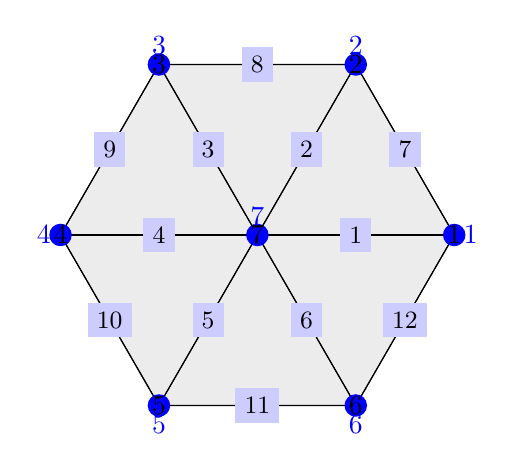
\begin{tikzpicture}[vertexStyle,edgePlain,faceStyle=nolabels]
    \def\r{2.5}
\tikzset{path/.style={double=red,double distance=1.3pt}}
\tikzset{edgeSpec/.style={edgeLabel,font=\small}}

\coordinate (Z) at (0,0);
\foreach \i in {1,...,6}{
    \coordinate (P\i) at (-60+60*\i:\r);
}

\draw[face=\faceColorSecond]
    \foreach \i/\j in {1/2,2/3,3/4,4/5,5/6,6/1}{
        (Z) -- (P\i) -- (P\j) -- cycle
    }
;


% Draw the edges separately, depending on the vertex-edge-paths that are active

% Edge 1, 4
\draw[edge,\ifdefined\cloverPath path\fi] 
    (Z) -- node[edgeSpec] {1} (P1)
    (Z) -- node[edgeSpec] {4} (P4);

% Edge 2, 3
\draw[edge,\ifdefined\cloverPath path\fi,\ifdefined\alphaPath path\fi] 
    (Z) -- node[edgeSpec] {2} (P2)
    (Z) -- node[edgeSpec] {3} (P3);

% Edge 5, 6
\draw[edge,\ifdefined\omegaPath path\fi,\ifdefined\cloverPath path\fi,\ifdefined\alphaPath path\fi]
    (Z) -- node[edgeSpec] {5} (P5)
    (Z) -- node[edgeSpec] {6} (P6);

% Edge 7
\draw[edge,\ifdefined\circlePath path\fi,\ifdefined\omegaPath path\fi,\ifdefined\cloverPath path\fi]
    (P1) -- node[edgeSpec] {7} (P2);

% Edge 8
\draw[edge,\ifdefined\circlePath path\fi]
    (P2) -- node[edgeSpec] {8} (P3);
% Edge 9
\draw[edge,\ifdefined\circlePath path\fi,\ifdefined\omegaPath path\fi,\ifdefined\cloverPath path\fi,\ifdefined\alphaPath path\fi]
    (P3) -- node[edgeSpec] {9} (P4);

% Edge 10
\draw[edge,\ifdefined\circlePath path\fi,\ifdefined\omegaPath path\fi,\ifdefined\alphaPath path\fi]
    (P4) -- node[edgeSpec] {10} (P5);

% Edge 11
\draw[edge,\ifdefined\circlePath path\fi,\ifdefined\cloverPath path\fi]
    (P5) -- node[edgeSpec] {11} (P6);

% Edge 12
\draw[edge,\ifdefined\circlePath path\fi,\ifdefined\omegaPath path\fi]
    (P6) -- node[edgeSpec] {12} (P1);




% Draw vertices
\foreach \p/\r/\n in {P1/right/1, P2/above/2, P3/above/3, P4/left/4, P5/below/5, P6/below/6, Z/above/7}{
    \vertexLabelR{\p}{\r}{\n}
}

\end{tikzpicture}

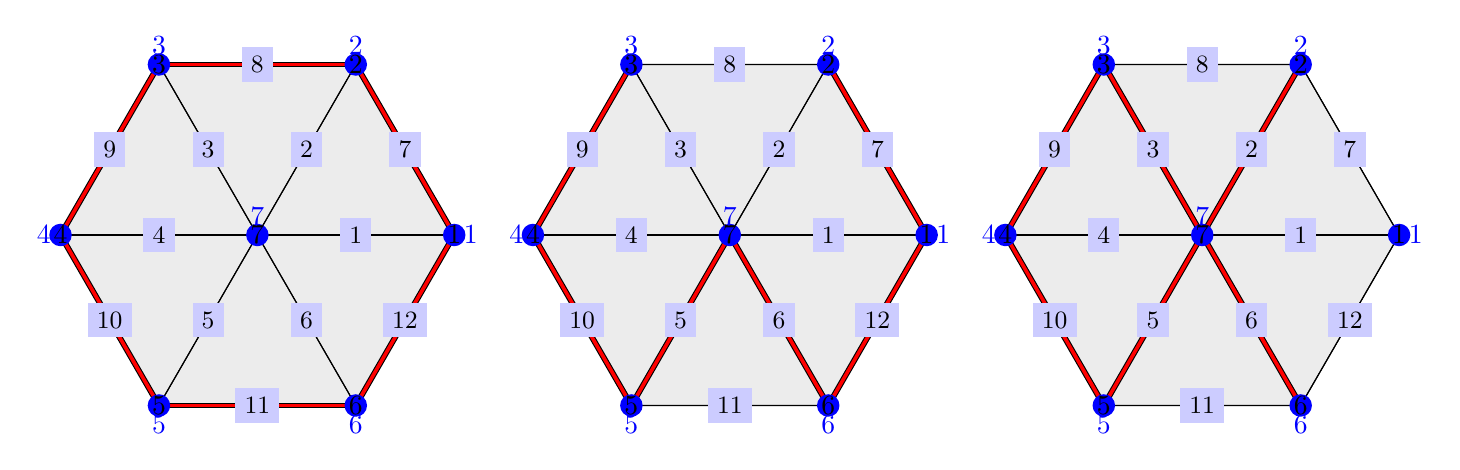
\begin{tikzpicture}[vertexStyle,edgePlain,faceStyle=nolabels]
    \begin{scope}
        \def\circlePath{1}
        \def\r{2.5}
\tikzset{path/.style={double=red,double distance=1.3pt}}
\tikzset{edgeSpec/.style={edgeLabel,font=\small}}

\coordinate (Z) at (0,0);
\foreach \i in {1,...,6}{
    \coordinate (P\i) at (-60+60*\i:\r);
}

\draw[face=\faceColorSecond]
    \foreach \i/\j in {1/2,2/3,3/4,4/5,5/6,6/1}{
        (Z) -- (P\i) -- (P\j) -- cycle
    }
;


% Draw the edges separately, depending on the vertex-edge-paths that are active

% Edge 1, 4
\draw[edge,\ifdefined\cloverPath path\fi] 
    (Z) -- node[edgeSpec] {1} (P1)
    (Z) -- node[edgeSpec] {4} (P4);

% Edge 2, 3
\draw[edge,\ifdefined\cloverPath path\fi,\ifdefined\alphaPath path\fi] 
    (Z) -- node[edgeSpec] {2} (P2)
    (Z) -- node[edgeSpec] {3} (P3);

% Edge 5, 6
\draw[edge,\ifdefined\omegaPath path\fi,\ifdefined\cloverPath path\fi,\ifdefined\alphaPath path\fi]
    (Z) -- node[edgeSpec] {5} (P5)
    (Z) -- node[edgeSpec] {6} (P6);

% Edge 7
\draw[edge,\ifdefined\circlePath path\fi,\ifdefined\omegaPath path\fi,\ifdefined\cloverPath path\fi]
    (P1) -- node[edgeSpec] {7} (P2);

% Edge 8
\draw[edge,\ifdefined\circlePath path\fi]
    (P2) -- node[edgeSpec] {8} (P3);
% Edge 9
\draw[edge,\ifdefined\circlePath path\fi,\ifdefined\omegaPath path\fi,\ifdefined\cloverPath path\fi,\ifdefined\alphaPath path\fi]
    (P3) -- node[edgeSpec] {9} (P4);

% Edge 10
\draw[edge,\ifdefined\circlePath path\fi,\ifdefined\omegaPath path\fi,\ifdefined\alphaPath path\fi]
    (P4) -- node[edgeSpec] {10} (P5);

% Edge 11
\draw[edge,\ifdefined\circlePath path\fi,\ifdefined\cloverPath path\fi]
    (P5) -- node[edgeSpec] {11} (P6);

% Edge 12
\draw[edge,\ifdefined\circlePath path\fi,\ifdefined\omegaPath path\fi]
    (P6) -- node[edgeSpec] {12} (P1);




% Draw vertices
\foreach \p/\r/\n in {P1/right/1, P2/above/2, P3/above/3, P4/left/4, P5/below/5, P6/below/6, Z/above/7}{
    \vertexLabelR{\p}{\r}{\n}
}

    \end{scope}
    \begin{scope}[xshift=6cm]
        \def\omegaPath{1}
        \def\r{2.5}
\tikzset{path/.style={double=red,double distance=1.3pt}}
\tikzset{edgeSpec/.style={edgeLabel,font=\small}}

\coordinate (Z) at (0,0);
\foreach \i in {1,...,6}{
    \coordinate (P\i) at (-60+60*\i:\r);
}

\draw[face=\faceColorSecond]
    \foreach \i/\j in {1/2,2/3,3/4,4/5,5/6,6/1}{
        (Z) -- (P\i) -- (P\j) -- cycle
    }
;


% Draw the edges separately, depending on the vertex-edge-paths that are active

% Edge 1, 4
\draw[edge,\ifdefined\cloverPath path\fi] 
    (Z) -- node[edgeSpec] {1} (P1)
    (Z) -- node[edgeSpec] {4} (P4);

% Edge 2, 3
\draw[edge,\ifdefined\cloverPath path\fi,\ifdefined\alphaPath path\fi] 
    (Z) -- node[edgeSpec] {2} (P2)
    (Z) -- node[edgeSpec] {3} (P3);

% Edge 5, 6
\draw[edge,\ifdefined\omegaPath path\fi,\ifdefined\cloverPath path\fi,\ifdefined\alphaPath path\fi]
    (Z) -- node[edgeSpec] {5} (P5)
    (Z) -- node[edgeSpec] {6} (P6);

% Edge 7
\draw[edge,\ifdefined\circlePath path\fi,\ifdefined\omegaPath path\fi,\ifdefined\cloverPath path\fi]
    (P1) -- node[edgeSpec] {7} (P2);

% Edge 8
\draw[edge,\ifdefined\circlePath path\fi]
    (P2) -- node[edgeSpec] {8} (P3);
% Edge 9
\draw[edge,\ifdefined\circlePath path\fi,\ifdefined\omegaPath path\fi,\ifdefined\cloverPath path\fi,\ifdefined\alphaPath path\fi]
    (P3) -- node[edgeSpec] {9} (P4);

% Edge 10
\draw[edge,\ifdefined\circlePath path\fi,\ifdefined\omegaPath path\fi,\ifdefined\alphaPath path\fi]
    (P4) -- node[edgeSpec] {10} (P5);

% Edge 11
\draw[edge,\ifdefined\circlePath path\fi,\ifdefined\cloverPath path\fi]
    (P5) -- node[edgeSpec] {11} (P6);

% Edge 12
\draw[edge,\ifdefined\circlePath path\fi,\ifdefined\omegaPath path\fi]
    (P6) -- node[edgeSpec] {12} (P1);




% Draw vertices
\foreach \p/\r/\n in {P1/right/1, P2/above/2, P3/above/3, P4/left/4, P5/below/5, P6/below/6, Z/above/7}{
    \vertexLabelR{\p}{\r}{\n}
}

    \end{scope}
    \begin{scope}[xshift=12cm]
        \def\alphaPath{1}
        \def\r{2.5}
\tikzset{path/.style={double=red,double distance=1.3pt}}
\tikzset{edgeSpec/.style={edgeLabel,font=\small}}

\coordinate (Z) at (0,0);
\foreach \i in {1,...,6}{
    \coordinate (P\i) at (-60+60*\i:\r);
}

\draw[face=\faceColorSecond]
    \foreach \i/\j in {1/2,2/3,3/4,4/5,5/6,6/1}{
        (Z) -- (P\i) -- (P\j) -- cycle
    }
;


% Draw the edges separately, depending on the vertex-edge-paths that are active

% Edge 1, 4
\draw[edge,\ifdefined\cloverPath path\fi] 
    (Z) -- node[edgeSpec] {1} (P1)
    (Z) -- node[edgeSpec] {4} (P4);

% Edge 2, 3
\draw[edge,\ifdefined\cloverPath path\fi,\ifdefined\alphaPath path\fi] 
    (Z) -- node[edgeSpec] {2} (P2)
    (Z) -- node[edgeSpec] {3} (P3);

% Edge 5, 6
\draw[edge,\ifdefined\omegaPath path\fi,\ifdefined\cloverPath path\fi,\ifdefined\alphaPath path\fi]
    (Z) -- node[edgeSpec] {5} (P5)
    (Z) -- node[edgeSpec] {6} (P6);

% Edge 7
\draw[edge,\ifdefined\circlePath path\fi,\ifdefined\omegaPath path\fi,\ifdefined\cloverPath path\fi]
    (P1) -- node[edgeSpec] {7} (P2);

% Edge 8
\draw[edge,\ifdefined\circlePath path\fi]
    (P2) -- node[edgeSpec] {8} (P3);
% Edge 9
\draw[edge,\ifdefined\circlePath path\fi,\ifdefined\omegaPath path\fi,\ifdefined\cloverPath path\fi,\ifdefined\alphaPath path\fi]
    (P3) -- node[edgeSpec] {9} (P4);

% Edge 10
\draw[edge,\ifdefined\circlePath path\fi,\ifdefined\omegaPath path\fi,\ifdefined\alphaPath path\fi]
    (P4) -- node[edgeSpec] {10} (P5);

% Edge 11
\draw[edge,\ifdefined\circlePath path\fi,\ifdefined\cloverPath path\fi]
    (P5) -- node[edgeSpec] {11} (P6);

% Edge 12
\draw[edge,\ifdefined\circlePath path\fi,\ifdefined\omegaPath path\fi]
    (P6) -- node[edgeSpec] {12} (P1);




% Draw vertices
\foreach \p/\r/\n in {P1/right/1, P2/above/2, P3/above/3, P4/left/4, P5/below/5, P6/below/6, Z/above/7}{
    \vertexLabelR{\p}{\r}{\n}
}

    \end{scope}
\end{tikzpicture}

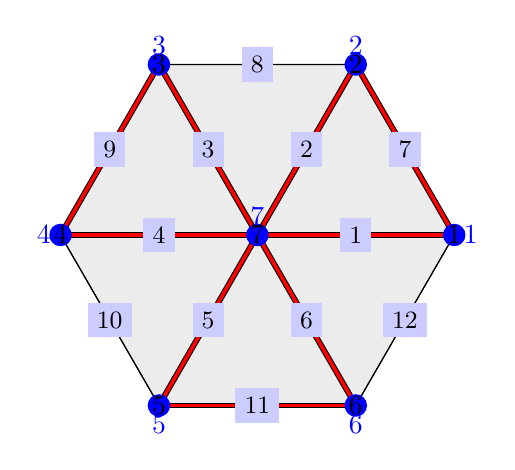
\begin{tikzpicture}[vertexStyle,edgePlain,faceStyle=nolabels]
    \def\cloverPath{1}
    \def\r{2.5}
\tikzset{path/.style={double=red,double distance=1.3pt}}
\tikzset{edgeSpec/.style={edgeLabel,font=\small}}

\coordinate (Z) at (0,0);
\foreach \i in {1,...,6}{
    \coordinate (P\i) at (-60+60*\i:\r);
}

\draw[face=\faceColorSecond]
    \foreach \i/\j in {1/2,2/3,3/4,4/5,5/6,6/1}{
        (Z) -- (P\i) -- (P\j) -- cycle
    }
;


% Draw the edges separately, depending on the vertex-edge-paths that are active

% Edge 1, 4
\draw[edge,\ifdefined\cloverPath path\fi] 
    (Z) -- node[edgeSpec] {1} (P1)
    (Z) -- node[edgeSpec] {4} (P4);

% Edge 2, 3
\draw[edge,\ifdefined\cloverPath path\fi,\ifdefined\alphaPath path\fi] 
    (Z) -- node[edgeSpec] {2} (P2)
    (Z) -- node[edgeSpec] {3} (P3);

% Edge 5, 6
\draw[edge,\ifdefined\omegaPath path\fi,\ifdefined\cloverPath path\fi,\ifdefined\alphaPath path\fi]
    (Z) -- node[edgeSpec] {5} (P5)
    (Z) -- node[edgeSpec] {6} (P6);

% Edge 7
\draw[edge,\ifdefined\circlePath path\fi,\ifdefined\omegaPath path\fi,\ifdefined\cloverPath path\fi]
    (P1) -- node[edgeSpec] {7} (P2);

% Edge 8
\draw[edge,\ifdefined\circlePath path\fi]
    (P2) -- node[edgeSpec] {8} (P3);
% Edge 9
\draw[edge,\ifdefined\circlePath path\fi,\ifdefined\omegaPath path\fi,\ifdefined\cloverPath path\fi,\ifdefined\alphaPath path\fi]
    (P3) -- node[edgeSpec] {9} (P4);

% Edge 10
\draw[edge,\ifdefined\circlePath path\fi,\ifdefined\omegaPath path\fi,\ifdefined\alphaPath path\fi]
    (P4) -- node[edgeSpec] {10} (P5);

% Edge 11
\draw[edge,\ifdefined\circlePath path\fi,\ifdefined\cloverPath path\fi]
    (P5) -- node[edgeSpec] {11} (P6);

% Edge 12
\draw[edge,\ifdefined\circlePath path\fi,\ifdefined\omegaPath path\fi]
    (P6) -- node[edgeSpec] {12} (P1);




% Draw vertices
\foreach \p/\r/\n in {P1/right/1, P2/above/2, P3/above/3, P4/left/4, P5/below/5, P6/below/6, Z/above/7}{
    \vertexLabelR{\p}{\r}{\n}
}

\end{tikzpicture}

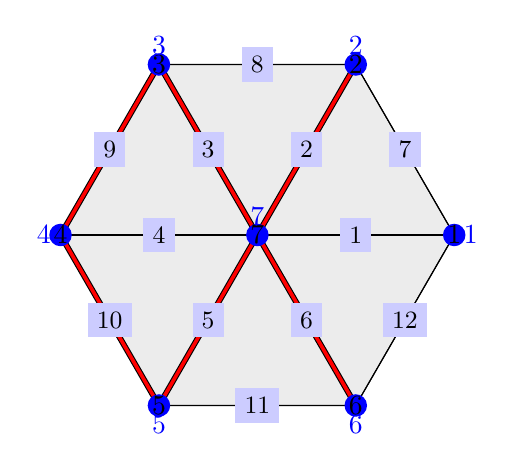
\begin{tikzpicture}[vertexStyle,edgePlain,faceStyle=nolabels]
    \def\alphaPath{1}
    \def\r{2.5}
\tikzset{path/.style={double=red,double distance=1.3pt}}
\tikzset{edgeSpec/.style={edgeLabel,font=\small}}

\coordinate (Z) at (0,0);
\foreach \i in {1,...,6}{
    \coordinate (P\i) at (-60+60*\i:\r);
}

\draw[face=\faceColorSecond]
    \foreach \i/\j in {1/2,2/3,3/4,4/5,5/6,6/1}{
        (Z) -- (P\i) -- (P\j) -- cycle
    }
;


% Draw the edges separately, depending on the vertex-edge-paths that are active

% Edge 1, 4
\draw[edge,\ifdefined\cloverPath path\fi] 
    (Z) -- node[edgeSpec] {1} (P1)
    (Z) -- node[edgeSpec] {4} (P4);

% Edge 2, 3
\draw[edge,\ifdefined\cloverPath path\fi,\ifdefined\alphaPath path\fi] 
    (Z) -- node[edgeSpec] {2} (P2)
    (Z) -- node[edgeSpec] {3} (P3);

% Edge 5, 6
\draw[edge,\ifdefined\omegaPath path\fi,\ifdefined\cloverPath path\fi,\ifdefined\alphaPath path\fi]
    (Z) -- node[edgeSpec] {5} (P5)
    (Z) -- node[edgeSpec] {6} (P6);

% Edge 7
\draw[edge,\ifdefined\circlePath path\fi,\ifdefined\omegaPath path\fi,\ifdefined\cloverPath path\fi]
    (P1) -- node[edgeSpec] {7} (P2);

% Edge 8
\draw[edge,\ifdefined\circlePath path\fi]
    (P2) -- node[edgeSpec] {8} (P3);
% Edge 9
\draw[edge,\ifdefined\circlePath path\fi,\ifdefined\omegaPath path\fi,\ifdefined\cloverPath path\fi,\ifdefined\alphaPath path\fi]
    (P3) -- node[edgeSpec] {9} (P4);

% Edge 10
\draw[edge,\ifdefined\circlePath path\fi,\ifdefined\omegaPath path\fi,\ifdefined\alphaPath path\fi]
    (P4) -- node[edgeSpec] {10} (P5);

% Edge 11
\draw[edge,\ifdefined\circlePath path\fi,\ifdefined\cloverPath path\fi]
    (P5) -- node[edgeSpec] {11} (P6);

% Edge 12
\draw[edge,\ifdefined\circlePath path\fi,\ifdefined\omegaPath path\fi]
    (P6) -- node[edgeSpec] {12} (P1);




% Draw vertices
\foreach \p/\r/\n in {P1/right/1, P2/above/2, P3/above/3, P4/left/4, P5/below/5, P6/below/6, Z/above/7}{
    \vertexLabelR{\p}{\r}{\n}
}

\end{tikzpicture}

\end{document} 
